\chapter{Introduction}

Ship handling is the task of precisely controlling a seafaring vessel’s movement using its propulsion and navigation systems. Ships move in a variety of marine environments - starting from shallow waters of a harbour, a vessel may navigate vast seas to a port across the ocean. They also navigate inland waterways such as rivers, canals, backwaters and creeks. More recently, developments in offshore wind farming, the oil and gas industry have necessitated regular visits to offshore structures located on continental shelves for construction and maintenance activities \parencite{halvorsen2012optimal}. 

%Navigation in marine environments just as in aviation requires the navigator to assimilate information of environmental forces at play. In 1955, the US Navy began researching head-up displays (HUD) to reduce complexity of aircraft instrumentation. HUDs were found helpful for piloting and by 1970s, the use of HUDs expanded beyond military aircraft into commercial aviation. 

%Handling a ship in varied environments is the job of a skilled seafarer who controls its movement precisely with a consideration of environmental forces such as wind, waves and current acting on the ship \parencite{wiki:seamanship}. 

It takes a skilled seafarer to handle a ship with accurate control \parencite{wiki:seamanship}. In addition to manoeuvring the vessel, natural forces acting on it (current, wind, waves) need to be accounted for. Traditionally, navigational-aid information such as prevailing weather conditions, charts, etc. have been presented using numerous display panels placed around the navigator in the ship bridge \parencite{vasiljevic2011augmented} with recent developments in instrumentation design featuring relatively minimal, less-cluttered designs \parencite{sauer2002effects}. This design change is a reflection of increasing automation trickling into maritime industrial processes \parencite{perunovic2011innovation}. 
 
As in aviation, modern maritime navigation requires the navigator to assimilate information from various sources. Use of head-up displays, however, is not yet commonplace in the latter \parencite{holder2011maritime}. It could be attributable to the maritime industry being a niche sector with a conservative attitude towards innovation \parencite{perunovic2011innovation}. Nevertheless, research studies can be found on maritime applications of augmented reality (\cite{hugues2010experimental}, \cite{vasiljevic2011augmented} \cite{okazaki2014development} and, \cite{von2014maritime}). Unsurprisingly, there has been a focus on augmenting vision with real-time information of the environment; potentially helping navigators perform the job more efficiently. 

%For example, overlaying the bridge-view of a ship with route way-points, distance to next way-point, local hazards, and navigational aids such as buoys, lighthouses. 

%The dynamic positioning system for example can be used to automatically position a vessel at a specific location. 

%
%, thus making display panels for position, thruster/propeller-related information more redundant than before.\ 

Few research studies can be found on the viability of mixed reality technologies to create simulation environments for training purposes. Ship simulations systems are currently the \textit{de facto} method of learning ship navigation. Various schools around the world setup simulation centers where generic principles of sea-faring can be learned and practiced. With increasing automation, the need for human-operation will reduce and so will the need to learn to do them manually. This research studies the feasibility of a training method to learn vessel operations in augmented reality on-board ships. 
%while also being driven by requirements for customizable instrument panels. 

\section{Research Questions}
Ship simulators are used by ship crew for learning, certification and, upkeep of operational skills. As simulations, they are approximations of the process after all. It can be conjectured that on-board training involving operation of a real vessel in actual conditions is advantageous as it allows for situated learning. 

Going by situated learning theory, manoeuvring a ship for example, is better learned by practising on an actual ship in real conditions than on simulators. However, a manoeuvre training programme that requires movement of an actual vessel comes at the cost of ship operation time and operational expenses in the form of fuel and machinery. Nevertheless, it provides hands-on experience of ship's movement behaviour in various weather conditions. Such a training should also result in better acquaintance with vessel-specific instrumentation. But it is difficult to set up training environments on-board since, environments in this context consist of large structures such as ports, natural landscapes, other vessels, offshore constructions etc.

A system of generating visual perception of large objects on-board is then desirable. It can be a solution to the non-trivial problem of setting up training environments. If such a system were capable of producing a convincing feeling of the presence of physical objects in the surrounding, it would enable on-board training in real environments enhanced by visuals of virtual objects.

With the intention of learning feasibility of using augmented reality for on-board training purposes, the following research questions were proposed.

%[before=\sffamily]
\begin{enumerate}
	\item \libertineSB{Which are operational scenarios where augmented reality could be used for on-board training?}
	\item How can augmented reality be realized on-board ships?
	\item What is the experience of navigating ships in augmented reality using state-of-the-art see-through display?
\end{enumerate}

\section{Research Approach}
A method of research devised by \cite{neerincx2008situated} called situated cognitive engineering (SCE) was employed in this study. SCE method separates a human-computer interaction research into three different phases namely derive, specify and evaluate (see Figure \ref{fig:sce}). Characteristic to each phase is the type of information that is gathered. This section contains a brief description of the phases and work performed in each of them. 

In the derive phase, the problem domain is analysed to create abstract definitions of operations that take place in it relevant to the topic of research. Further, human physiological factors that can be influential to the design, technological possibilities for implementation are examined. Interviewing licensed mariners and professionals in the maritime industry was the \textit{modus operandi} to outline operational demands. Additionally, a literature survey on applications of augmented reality in maritime sector provided insight into areas of research yet unexplored in this domain. Further, the literature survey also led to an understanding of trade-offs of various technical options for implementation of augmented reality on-board.

\begin{figure}
	\centering
	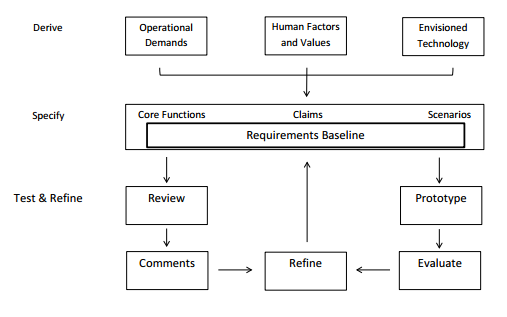
\includegraphics[width=0.80\linewidth]{situatedcognitive}
	\caption{Situated Cognitive Engineering Method \parencite{neerincx2008situated}}
	\label{fig:sce}
\end{figure}

The specification phase is based on information from derive phase. In this phase we chalk out a use case scenario for the design solution, specify functional requirements for the system and make claims on consequences of its use. Previously in the derive phase, a few different on-board training possibilities were considered and grouped into the categories - manoeuvring, navigation and emergency response training. A choice was made between them going into the specification phase. Manoeuvre training was chosen as the scenario for prototyping and evaluation. This decision was driven by a growing market demand for on-board training solutions for manoeuvring and, feasibility of prototyping within the available time-frame. Accordingly, Chapter \ref{chap:specification} titled Specification sketches the use-case for a station-keeping (a ship manoeuvre) scenario using augmented reality. 

Chapter 4 named Evaluation describes the artefact that was developed, an experiment designed to test the claims and, discusses results and conclusion of the experiment. The final prototype consisted of head-mounted see-through display and outside-in head tracking to generate augmented reality. It accepted input from a maritime simulator which provided for interaction within the augmented reality environment. Even though the prototype is capable accepting position data from a real ship in real-time, its evaluation was made on a maritime simulator developed by VSTEP B.V., Rotterdam. The set-up allowed for precise control of weather conditions in the simulation. More importantly it enabled the comparison of quality of depth perception in augmented reality with that in a modern maritime simulator.

%Accordingly, this report has been structured to describe the three phases of this research outlined by the method. Chapter 2 named Foundation first describes so-called operational demands that define requirements of the problem at an abstract level. It goes on to describe existing knowledge of human anatomical factors that can be leveraged in designing a solution to the problem. The chapter ends with a survey of possible technological solutions, stating also their strengths and weaknesses. Chapter 3 named Specification sketches a real-life scenario in which the artefact could possibly be used. It lists formal requirements for the software system and makes claims about consequences of its use. 



\section{Augmented Reality}
\label{sec:augreal}
This section introduces the concept of augmented reality for a novice reader. It is in good order to have a clear understanding of the primary technology being researched before delving into details of its design and implementation. The information is elementary, readers familiar with the term 'augmented reality' and similar technologies will find the information basic. All the same, an overview of the technological domain can be useful to place the research study in the broader perspective.

\begin{figure}
	\centering
	\includegraphics[width=\linewidth]{mrcontinuum3}
	\caption{Mixed Reality Continuum (Adapted from \cite{milgram1995augmented})}
	\label{fig:mixedrealitycontinuum}
\end{figure}

Mixed reality is the merging of virtual and real worlds in which physical and digital objects co-exist and interact in real time \parencite{wiki:mixedreality}. Distinctions have been made between various types of applications in this realm based on the amount of virtual content in the mix. \cite{milgram1995augmented} drew up a continuum (figure \ref{fig:mixedrealitycontinuum}) characterising different mixed reality environments. Completely real and completely virtual environments bring up far ends of the continuum with different levels of virtuality in between. Virtual reality on the far right of the spectrum refers to the experience in which users' perception of reality is influenced to create the feeling of immersion in a technologically-mediated world \parencite{steuer1992defining}. This type of mixed reality features  digital visuals often composed of entirely fictional environments. 

Augmented reality refers to systems that feature predominantly real environments whose perception may be altered to add information not readily available to the user. In a survey paper on augmented reality, \cite{azuma1997survey} identified the technology to have the following three characteristics: 
\begin{itemize}[noitemsep]
	\renewcommand{\labelitemi}{\scalebox{.9}{\tiny\listsymb}}
	\item It combines real and virtual 
	\item Is interactive in real time
	\item Is registered in three dimensions
\end{itemize} 

%\begin{figure}
%	\centering
%	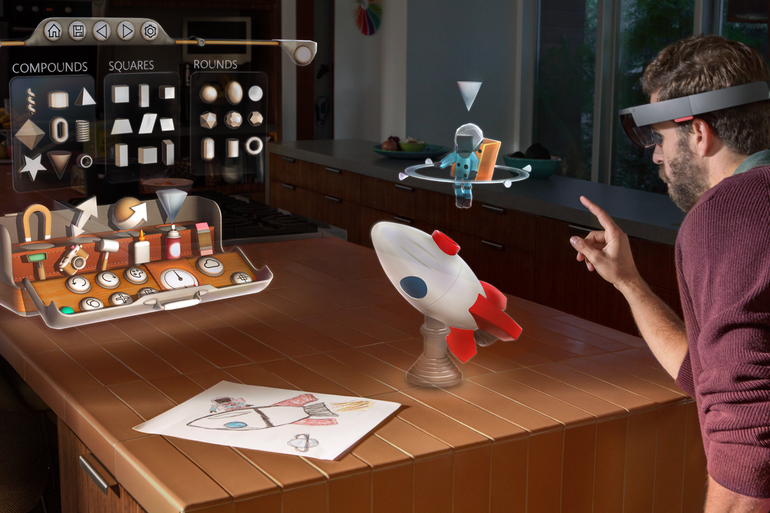
\includegraphics[width=0.75\linewidth]{hololensAR}
%	\caption{Conceptual depiction of augmented reality used for design visualization}
%	\label{fig:augreal}
%\end{figure}

%Further, some factors have been identified that help distinguish between different mixed reality systems: extent of world knowledge (whether the augmentation takes place in a modeled world or not), reproduction fidelity (quality of display of the real/virtual objects) and extent of presence metaphor (extent to which user feels they are present in the displayed scene themselves). A detailed description of mixed reality displays and differences in their characteristics can be found in \cite{milgram1995augmented}. 

In general terms, mixed reality is an emerging technology which can be used to display virtual objects merged with real world views. It has been found to be useful in job scenarios that require execution of complex tasks \parencite{henderson2011exploring}. A use case that has been explored in the real-world is assembly and maintenance of equipment. 3-D virtual job-support guides overlaid on see-through images of actual equipment obviates the need to look away in order to refer to a manual. It was found that virtual guides help users perform ship building and maintenance tasks in almost half the usual time \parencite{henderson2011exploring}. 

%It is also used in context of 3D visualizations of designs in real world spaces.

